
\subsubsection{16.10.14}

\begin{enumerate}
	\item Time of beginning and ending of meeting:
	17:00 - 21:00
	\item Purposes of meeting:
	\begin{enumerate}
	  \item To connect controller for servomotors and link servomotor that rotates gripper for balls to it .
	  
	  \item To include to the programme of control robot control gripper for balls.
	  
	  \item To improve the lift.
	  
    \end{enumerate}
	\item Work that has been done:
	\begin{enumerate}
	  \item To date it was bought aluminium strip 100 x 4 x 0.3cm for creating transverse beams for connection guides of the lift and aluminium axle length 100 cm and a diameter 8 mm for creating crossbars.
      
      \item Strip wac cut at 4 segments with neded leigth. It was decided to buy L-shaped profile and cut to it on the corners of needed size for installation transverse beams to guides.
      
      \item Axle was enough for 4 crossbars of the required 6. Two axles were installed to lift with help of elements from Tetrix set. They were made holes for another one axis but it wasn't installed to the lift. It was decided not to install the last crossbar for the top pair of slats because we have not yet figured out how to do it and it would make difficult the improvement of lift.
      
      \item Controller for servos was installed and it was connected to servo of continuous rotation. This servo rotates gripper of the balls.
      
      \begin{figure}[H]
      	\begin{minipage}[h]{1\linewidth}
      		\center {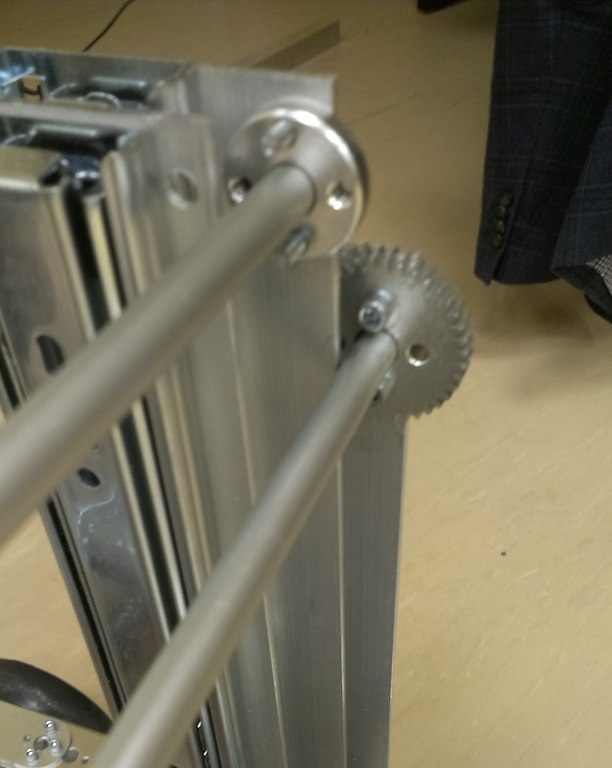
\includegraphics[scale=0.3]{days/16.10.14/images/01}}
      		\caption{Crossbars that were installed to robot} 
      	\end{minipage}
      	%\hfill
      %	\begin{minipage}[h]{0.5\linewidth}
     % 		\center{
\includegraphics[scale=0.4]{days/16.10.14/images/02}}
      %		\caption{Контроллер сервоприводов}
      %	\end{minipage}
      \end{figure}
      
    \end{enumerate}
    
	\item Results: 
	\begin{enumerate}
	  \item Controller for servo was installed.
	  
      \item The programme of control servo wasn't wrote.
      
      \item Aluminium strip was cut at the beams with needed length.
      
      \item Axle was cut at crossbars.
      
    \end{enumerate}
    
	\item Tasks for the next meetings:
	\begin{enumerate}
	  \item To buy another one aluminium axle and make the rest of crossbars.
	  
	  \item To buy L-shaped profile and to cut it into the corners for fixing beams to the lift.

    \end{enumerate}     
\end{enumerate}
\fillpage
